%Este trabalho está licenciado sob a Licença Atribuição-CompartilhaIgual 4.0 Internacional Creative Commons. Para visualizar uma cópia desta licença, visite http://creativecommons.org/licenses/by-sa/4.0/deed.pt_BR ou mande uma carta para Creative Commons, PO Box 1866, Mountain View, CA 94042, USA.

\chapter{Aplicações da integral}\label{cap_apint}
\thispagestyle{fancy}

\section{Cálculo de áreas}\label{cap_apint_sec_areas}

% \begin{flushright}
%   [Vídeo] | [Áudio] | \href{https://phkonzen.github.io/notas/contato.html}{[Contatar]}
% \end{flushright}

A integral definida $\int_a^b f(x)\,dx$ está associada a área entre o gráfico da função $f$ e o eixo das abscissas no intervalo $[a,b]$ (consulte Figura \ref{fig:apint_arealiq}). Ocorre que \hl{se $f$ for não negativa, então $\int_a^b f(x)\,dx \geq 0$}. \hl{Se $f$ for negativa, então $\int_a^b f(x)\,dx < 0$}. Por isso, dizemos que \hl{$\int_a^b f(x)\,dx$ é a \emph{área líquida} (ou com sinal) entre o gráfico de $f$ e o eixo das abscissas}.

\begin{figure}[H]
  \centering
  \includegraphics[width=0.7\textwidth]{./cap_apint/dados/fig_apint_arealiq/fig}
  \caption{Integral definida e a área com sinal.}
  \label{fig:apint_arealiq}
\end{figure}

\begin{ex}\label{ex:apint_arealiq}
  Vamos calcular a área total entre o gráfico de $f(x) = (x-1)^3$ e o eixo das abscissas, restrito ao intervalo $[0, 2]$.

  \begin{figure}[H]
    \centering
    \includegraphics[width=0.7\textwidth]{./cap_apint/dados/fig_ex_apint_arealiq/fig}
    \caption{Área total entre o gráfico de $f(x) = (x-1)^3$ e o eixo das abscissas para $x\in [0, 2]$.}
    \label{fig:ex_apint_arealiq}
  \end{figure}  

  Começamos fazendo o estudo de sinal de $f$ no intervalo. Como $x-1 \leq 0$ para $x\leq 1$ e, $x-1\geq 0$ para $x \geq 1$, temos que $f(x)<0$ em $[0, 1]$ e $f(x)>0$ em $[1, 2]$. Logo, a área total é dada por
  \begin{equation}
    A = -\int_0^1f(x)\,dx + \int_1^2f(x)\,dx.
  \end{equation}
  
  Agora, usando a substituição $u=x-1$, temos $du = dx$ e segue que
  \begin{align}
    \int f(x)\,dx &= \int (x-1)^3\,dx \\
                  &= \int u^3\,du \\
                  &= \frac{u^4}{4} + C \\
                  &= \frac{(x-1)^4}{4} + C.
  \end{align}

  Então, do Teorema Fundamental do Cálculo, obtemos
  \begin{align}
    A &= -\int_0^1f(x)\,dx + \int_1^2f(x)\,dx \\
      &= -\left[\frac{(x-1)^4}{4}\right]_0^1 + \left[\frac{(x-1)^4}{4}\right]_1^2 \\
      &= -\left[\frac{(1-1)^4}{4} - \frac{(0-1)^4}{4}\right] + \left[\frac{(2-1)^4}{4} - \frac{(1-1)^4}{4}\right] \\
      &= \frac{1}{4} + \frac{1}{4} = \frac{1}{2}.
  \end{align}

  \ifispython
  Com {\python}+{\sympy}, podemos computar a área com os seguintes comandos:
    \begin{lstlisting}
      In : from sympy import *
      ...: x = symbols('x')
      ...: f = (x-1)**3
      ...: A = integrate(f, (x,0,1))
      ...: B = integrate(f, (x,1,2))
      ...: -A+B
      Out: 1/2
    \end{lstlisting}
    \fi  
\end{ex}

\subsection{Áreas entre curvas}

\begin{flushright}
  [Vídeo] | [Áudio] | \href{https://phkonzen.github.io/notas/contato.html}{[Contatar]}
\end{flushright}

Observamos que se $f(x)\geq g(x)$ no intervalo $[a, b]$, então
\begin{equation}
  \int_a^b f(x)-g(x)\,dx = \int_a^bf(x)\,dx - \int_a^bg(x)\,dx
\end{equation}
corresponde à área entre as curvas $y = f(x)$ e $y = g(x)$ restritas ao intervalo $[a,b]$. Ou seja, fazendo $h(x) = f(x)-g(x)$, temos que
\begin{equation}
  \int_a^bh(x)\,dx
\end{equation}
é a área entre essas curvas restritas ao intervalo $[a, b]$. Ainda, se $f(x)\leq g(x)$, entre a área entre elas é dada por
\begin{equation}
  -\int_a^bh(x)\,dx = \int_a^bg(x)\,dx - \int_a^bf(x)\,dx.
\end{equation}

\begin{ex}\label{ex:apint_areacurvas}
  Vamos calcular a área entre as curvas $y = (x-1)^3$, $y = x-1$, $x=0$ e $x=2$.

  \begin{figure}[H]
    \centering
    \includegraphics[width=0.7\textwidth]{./cap_apint/dados/fig_ex_apint_areacurvas/fig}
    \caption{Área entre as curvas $y = (x-1)^3$, $y = x-1$, $x=0$ e $x=2$.}
    \label{fig:ex_apint_areacurvas}
  \end{figure}  

  Começamos definindo $h(x) = (x-1)^3 - (x-1)$. A fim de fazermos o estudo de sinal de $h$, identificamos seus zeros.
  \begin{align}
    h(x) &= (x-1)^3-(x-1) \\
         &= (x-1)\left[(x-1)^2-1\right] \\
         &= (x-1)(x^2-2x) \\
         &= (x-1)\cdot x\cdot (x-2).
  \end{align}
  Ou seja, $x_1=0$, $x_2=1$ e $x_3=2$ são as raízes de $h$. Daí, segue seu estudo de sinal:
  \begin{center}
    \begin{tabular}{l|c|c}
              & $0<x<1$ & $1<x<2$ \\\hline
      $(x-1)$ &   -     &    +    \\
      $x$     &   +     &    +    \\
      $(x-2)$ &   -     &    -    \\\hline
      $h(x)$  &   +     &    -    \\\hline
    \end{tabular}
  \end{center}
  Assim, temos que a área desejada pode ser calculada como
  \begin{equation}
    A = \int_0^1 h(x)\,dx - \int_1^2 h(x)\,dx.
  \end{equation}

  Agora, calculamos a integral de $h$, i.e.
  \begin{align}
    \int h(x)\,dx &= \int (x-1)^3-(x-1)\,dx \\
                  &= \int (x-1)^3\,dx - \int x\,dx + \int\,dx \\
                  &= \frac{(x-1)^4}{4} - \frac{x^2}{2} + x + C.
  \end{align}

  Por fim, do Teorema Fundamental do Cálculo, obtemos
  \begin{align}
    A &= \int_0^1 h(x)\,dx - \int_1^2 h(x)\,dx \\
      &= \left[\frac{(x-1)^4}{4} - \frac{x^2}{2} + x\right]_0^1 - \left[\frac{(x-1)^4}{4} - \frac{x^2}{2} + x\right]_1^2 \\
      &= -\frac{1}{2}+1-\frac{1}{4}-\left(\frac{1}{4}-2+2+\frac{1}{2}-1\right) \\
      &= \frac{1}{2}.
  \end{align}
  
  \ifispython
  Com o {\python}+{\sympy}, podemos computar a área com os seguintes comandos:
  \begin{lstlisting}
    In : from sympy import *
    ...: x = symbols('x')
    ...: f = (x-1)**3 - (x-1)
    ...: integrate(abs(f), (x,0,2))
    Out: 1/2
  \end{lstlisting}
  \fi  
\end{ex}

\subsubsection{Calculando áreas em função de $y$}

\begin{ex}
  Calcule a área determinada pelas curvas $x = y^2$ e $y = 2 - x$.

  \begin{figure}[H]
    \centering
    \includegraphics[width=0.7\textwidth]{./cap_apint/dados/fig_ex_apint_areacurvasy/fig}
    \caption{Área determinada pelas curvas $x = y^2$ e $y = 2 - x$.}
    \label{fig:ex_apint_areacurvasy}
  \end{figure}

  Uma das formas mais práticas de calcular esta área é integrando em relação a $y$. Para isso, precisamos que as curvas sejam descritas por funções de $x$ em $y$. A parábola $x = y^2$ já está escrita como tal, e a reta $y = 2 - x$ é equivalente a $x = 2 - y$. Com isso, temos que a área determinada por estas curvas tem medida
  \begin{align}
    \int_{-2}^1 \left[(2-y) - (y^2)\right]\,dy &= \int_{-2}^1 2-y-y^2\,dy\\
                                               &= \left. 2y-\frac{y^2}{2}-\frac{y^3}{3}\right|_{-2}^1\\
                                               &= \frac{7}{6} + \frac{10}{3}\\
                                               &=\frac{9}{2}
  \end{align}
  
  \ifispython
  Com o {\python}+{\sympy}, podemos computar a área com os seguintes comandos:
  \begin{lstlisting}
    In : from sympy import *
    ...: y = symbols('y')
    ...: f = 2 - y - y**2
    ...: integrate(f, (y, -2, 1))
    Out: 9/2
  \end{lstlisting}
  \fi  
\end{ex}

\subsection{Exercícios resolvidos}

\begin{exeresol}
  Cálculo a área entre a reta $y=1$ e o gráfico de $f(x)=x^2$ restritas ao intervalo $[0,1]$.
\end{exeresol}
\begin{resol}
  Observamos que a medida desta área corresponde à área do quadrado $\{0\leq x \leq 1\}\times \{0\leq y \leq 1\}$ descontada a área sob o gráfico de $f(x)=x^2$ restrita ao intervalo $[0,1]$. Isto é,
  \begin{align}
    A &= 1 - \int_0^1 x^2\,dx\\
      &= 1 - \left[\frac{x^3}{3}\right]_0^1\\
      &= 1 - \frac{2}{3} = \frac{1}{3}.
  \end{align}
\end{resol}

\begin{exeresol}
  Calcule a área entre as curvas $y=x^2$, $y=x$, $x=0$ e $x=1$.
\end{exeresol}
\begin{resol}
  O problema é equivalente a calcular a área entre os gráficos das funções $f(x)=x$ e $g(x)=x^2$ restritas ao intervalo $[0,1]$. Como $f(x)\geq g(x)$ neste intervalo, temos
  \begin{align}
    A &= \int_0^1 f(x)-g(x)\,dx\\
      &= \int_0^1 x-x^2\,dx\\
      &= \left.\frac{x^2}{2}-\frac{x^3}{3}\right|_0^1\\
      &= \frac{1}{6}.
  \end{align}
\end{resol}

\begin{exeresol}
  Calcule a área entre o gráfico de $f(x) = x^3-x$ e o eixo das abscissas no intervalo $[-1,1]$.
\end{exeresol}
\begin{resol}
  Para calcularmos a área entre o gráfico de $f(x)$ e o eixo das abscissas no intervalo $[-1,1]$, fazemos:
  \begin{enumerate}[1.]
  \item O estudo de sinal de $f$ no intervalo $[-1,1]$.
    \begin{enumerate}
    \item Cálculo das raízes de $f$ no intervalo $[-1,1]$.
      \begin{align}
        x^3-x=0 &\Rightarrow x(x^2-1)=0\\
                &\Rightarrow x(x-1)(x+1)=0\\
                &\Rightarrow x=-1\text{ ou }x=0\text{ ou }x=1.
      \end{align}
    \item Os sinais de $f(x)$.
      \begin{align}
        -1\leq x \leq 0 \Rightarrow f(x)\geq 0\\
        0\leq x \leq 1 \Rightarrow f(x)\leq 0.
      \end{align}
    \end{enumerate}
  \item Cálculo da área usando integrais definidas.
    \begin{enumerate}
    \item Cálculo da integral indefinida.
      \begin{align}
        \int f(x)\,dx &= \int x^3-x\,dx\\
                      &= \int x^3\,dx - \int x\,dx\\
                      &= \frac{x^4}{4} - \frac{x^2}{2} + C.
      \end{align}
    \item Cálculo da área.
    \begin{align}
      A &= \int_{-1}^0 f(x)\,dx - \int_{0}^{1} f(x)\,dx \\
        &= \left[\frac{x^4}{4} - \frac{x^2}{2}\right]_{-1}^0 - \left[\frac{x^4}{4} - \frac{x^2}{2}\right]_{0}^1\\
        &= \frac{1}{2}.
    \end{align}
    \end{enumerate}
  \end{enumerate}

  \ifispython
  Com {\python}+{\sympy}, podemos fazer o estudo de sinal de $f$ com os seguintes comandos
  \begin{lstlisting}
    In : from sympy import *
    ...: x = symbols('x')
    ...: f = lambda x: x**3 - x
    ...: reduce_inequalities(f(x)>=0)
    Out: ((-1 <= x) & (x <= 0)) | ((1 <= x) & (x < oo))
  \end{lstlisting}
  E, então, computamos a área com
  \begin{lstlisting}
    In : A = integrate(f(x), (x, -1, 0)) 
    ...: B = integrate(f(x), (x, 0, 1))
    ...: A - B
    Out: 1/2 
  \end{lstlisting}
  \fi
\end{resol}

\subsection{Exercícios}

\begin{exer}
  Calcule a área entre o gráfico de $y = x^2-1$ e o eixo das abscissas, restrita ao intervalo $[-1, 1]$.
\end{exer}
\begin{resp}
  $4/3$
\end{resp}

\begin{exer}
  Calcule a área entre o gráfico de $y = x^2-1$ e o eixo das abscissas, restrita ao intervalo $[-1, 2]$.
\end{exer}
\begin{resp}
  $8/3$
\end{resp}

\begin{exer}
  Calcule a área entre o gráfico de $f(x)=x^3$ e a reta $y=1$ restritas ao intervalo $[-1,1]$.
\end{exer}
\begin{resp}
  $2$
\end{resp}

\begin{exer}
  Calcule a área entre as curvas $y=x$, $y=x^2$, $x=0$ e $x=2$.
\end{exer}
\begin{resp}
  $1$
\end{resp}

\begin{exer}
  Calcule a área determinada pelas curvas $x=y^2$ e $y = x - 2$.
\end{exer}
\begin{resp}
  $9/2$
\end{resp}

\section{Volumes por fatiamento e rotação}\label{cap_apint_sec_volfat}

\begin{flushright}
  [Vídeo] | [Áudio] | \href{https://phkonzen.github.io/notas/contato.html}{[Contatar]}
\end{flushright}

\emconstrucao

\subsection{Exercícios resolvidos}

% \begin{flushright}
%   [Vídeo] | [Áudio] | \href{https://phkonzen.github.io/notas/contato.html}{[Contatar]}
% \end{flushright}

\badgeConstrucao

\subsection{Exercícios}

% \begin{flushright}
%   [Vídeo] | [Áudio] | \href{https://phkonzen.github.io/notas/contato.html}{[Contatar]}
% \end{flushright}

\badgeConstrucao

\section{Problema de valor inicial}\label{cap_apint_sec_pvi}

% \begin{flushright}
%   [Vídeo] | [Áudio] | \href{https://phkonzen.github.io/notas/contato.html}{[Contatar]}
% \end{flushright}

\badgeConstrucao

\subsection{Exercícios resolvidos}

% \begin{flushright}
%   [Vídeo] | [Áudio] | \href{https://phkonzen.github.io/notas/contato.html}{[Contatar]}
% \end{flushright}

\badgeConstrucao

\subsection{Exercícios}

% \begin{flushright}
%   [Vídeo] | [Áudio] | \href{https://phkonzen.github.io/notas/contato.html}{[Contatar]}
% \end{flushright}

\badgeConstrucao
